\documentclass{beamer}

\usepackage[ngerman]{babel}
\usepackage[utf8x]{inputenc}
\usepackage{amsmath,amsfonts,amssymb}
\usepackage{tikz}
\usepackage{graphicx}
\usepackage{eurosym}

\usetikzlibrary{shapes,arrows,positioning,hobby,decorations.markings,fit,backgrounds,calc}

%\usetheme{Singapore}
\setbeamercovered{transparent}

\setbeamertemplate{section in toc}[sections numbered]
\setbeamertemplate{subsection in toc}[subsections numbered]
\setbeamertemplate{subsubsection in toc}[subsubsections numbered]

\newcommand{\btVFill}{\vskip0pt plus 1filll}

\newcommand\subsectnum{%
  \number\numexpr \insertpagenumber-\insertsubsectionstartpage+1\relax.~%
}

\begin{document}
\title{IOT - Remote}   
\author{Eike Florian Petersen / Michael H} %TODO Ich weiß deinen Nachnamen nicht 
\date{\today}

\frame{\titlepage

\begin{minipage}{-0mm}
\hspace*{-1.3cm}
  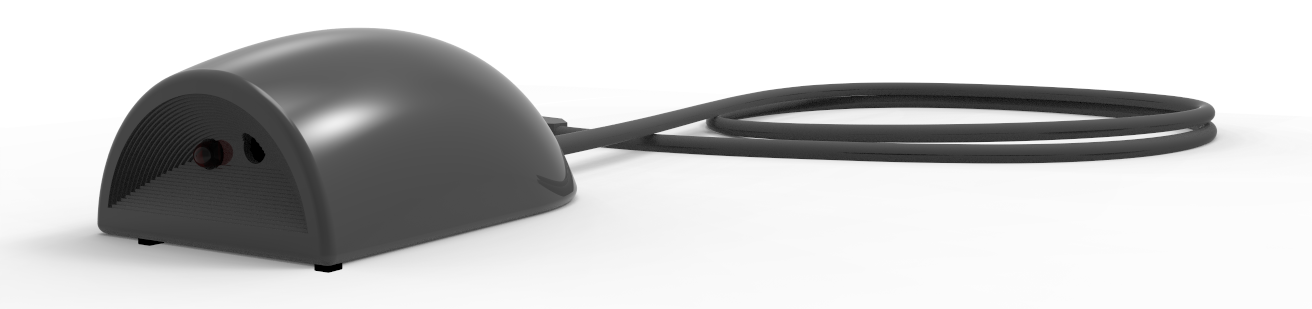
\includegraphics[width=13.5cm]{1_title}
\end{minipage}
}

\frame{\frametitle{Inhaltsverzeichnis}\tableofcontents} 


\section {Motivation / Aufgaben}
\frame {\frametitle{\thesection.~\insertsection}%\thesection.\thesubsection~\insertsection~- \insertsubsection}
Motivation:\\
Es soll eine frei konfigurierbare IoT-Infrarot Schnittstelle entstehen, welche außer dem Sender und seiner Stromversorgung keine weitere zusätzliche Hardware benötigt. Das erstrebte Ziel hebt sich von älteren Produkten der Firma Logitech aufgrund seiner nicht benötigten zweiten Hardwarekomponente (Fernbedienung) ab. Gleiches strebt auch Logitech mit dem MyHarmony Hub (aktuell \EUR{129,00}) an.\\
~\\
Aufgaben:\\
\begin{itemize}
	\item WiFi Einstellungen hinterlegen
	\item Fallback in AP Modus
	\item Webserver
	\item Steuerung des ESP8266 über Website (Feedback)
	\item Erfassen, Speichern und Ausgabe von Infrarot-Signalen (38kHz)
\end{itemize}
}
% Häufige Probleme mit dem Hub und der IOs / Android Anwendung, so wie später auslaufender Support von bestimmten Versionen von iOS und Android wird durch das Nutzen eines Webservers vorgebeugt


%\subsection {Konzept, Arten}
%\frame {\frametitle{\thesection.\thesubsection~\insertsection~- \insertsubsection}
%~\\
%Ein Tablespace (deutsch Tabellenraum) bezeichnet einen Speicherort (ein oder mehrere Dateien), in dem Tabellen, Indizes und andere Datenobjekte abgelegt werden. Er dient zur Trennung der logischen und physischen Speicherung.\\
%~\\
%Arten des Dateizugriffs$^1$:\\
%\begin{itemize} 
%\item SMS - `Operation' System Managed Storage
%\item DMS - Database Managed Storage
%\end{itemize}
%\begin{minipage}{6cm}
%Tablespace Arten in Oracle$^2$:
%\begin{itemize} 
%\item System Tablespace
%\item Sysaux Tablespace
%\item Rollback- / Undo Tablespace
%\item Tablespace für temporäre Daten
%\end{itemize}
%\btVFill \tiny
%~\\
%~\\
%Quellen: \\
%1 https://de.wikipedia.org/wiki/Tablespace\\
%2 http://docs.oracle.com/cd/B19306\_01/server.102/b14220/physical.htm\#i2006
%\end{minipage}
%\vspace{7mm}
%\begin{minipage}{4mm}
%  \includegraphics[width=4.6cm]{cncpt037}
%\end{minipage}
%}

\section {Bauteilliste}
\frame {\frametitle{\thesection.~\insertsection}
\begin{itemize}
	\item Mikrocontroller: ESP8266
	\item linearer Spannungsregler: LM1117-3V3 \\ (4.75V - 10V, max. 800 mA $\rightarrow$ 3.3V)
	\item Zwei Kondensatoren: 10 $\mu$F, 100nF
	\item IR-Diode: 1,5V / 80mA
	\item Vorwiderstand für IR-Diode: 22 Ohm
	\item IR-Fotodiode: TSOP4838 für die Trägerfrequenz 38kHz \\ (TSOP48.. in 30, 33, 36, 36.7, 38, 40, 50kHz)
	\item USB-to-UART-Programmierer: PL2303 \\ (Vss-Out = 5V)
\end{itemize}
}

\section {Schaltplan}
\frame {\frametitle{\thesection.~\insertsection}
\begin{minipage}{-0mm}
  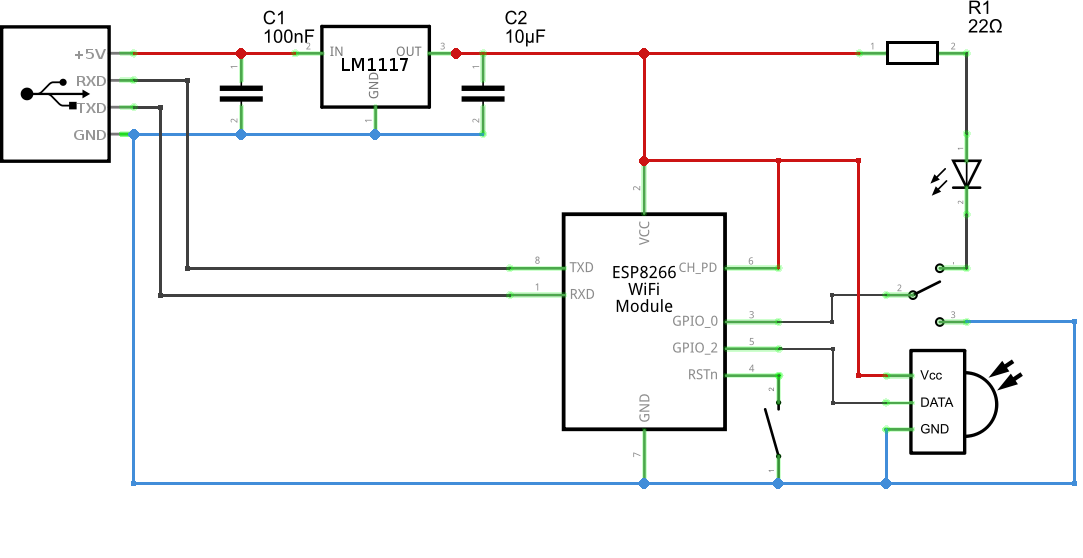
\includegraphics[width=11cm]{3_circuit_layout}
\end{minipage}
}

\section {Programm}
\subsection{EEPROM}
\frame {\frametitle{\thesection.\thesubsection~\insertsection~- \insertsubsection}
Lesen :\\
~ EEPROM.read(bytenr);\\~\\
Schreiben:\\
~ EEPROM.write(bytenr, 0);\\
~ EEPROM.write(bytenr, value);\\
~ \\
\begin{tikzpicture}
%Erster Block
\draw (0,0) -- (1,0) (1,1) --  (0,1) -- (0,0);
\draw (2,0) -- (3,0)  -- (3,1) --  (2,1);
\draw[loosely dotted] (2,1) -- (1,1);
\draw[loosely dotted] (2,0) -- (1,0);
\node[text width=4cm] at (2.4,1.2) {0};
\node[text width=4cm] at (4.3,1.2) {96};
\node[text width=4cm] at (2.5,0.45) {WiFi-Settings};
%Zweiter Block
\draw (4,0) -- (5,0) -- (5,1) --  (4,1) -- (4,0);
\draw (5,0) -- (6,0)  (6,1) --  (5,1) -- (5,0);
\draw (7,0) -- (8,0)  -- (8,1) --  (7,1);
\draw[loosely dotted] (6,1) -- (7,1);
\draw[loosely dotted] (6,0) -- (7,0);
\node[text width=4cm] at (6.2,1.2) {150};
\node[text width=4cm] at (7.2,1.2) {151};
\node[text width=4cm] at (9.2,1.2) {4095};

\node[text width=4cm] at (6.05,0.45) {\footnotesize Anzahl};
\node[text width=4cm] at (7.7,0.45) {IR-Codes};
% Detailansicht von IR-Codes

\draw (1,-2) -- (2,-2) -- (2,-1) --  (1,-1) -- (1,-2);
\draw (2,-2) -- (3,-2)  (3,-1) --  (2,-1) -- (2,-2);
\draw (4,-2) -- (5,-2)  -- (5,-1) --  (4,-1);
\draw[loosely dotted] (3,-1) -- (4,-1);
\draw[loosely dotted] (3,-2) -- (4,-2);
\node[text width=4cm] at (3.05,-1.55) {\footnotesize Anzahl};
\node[text width=4cm] at (4.2,-1.55) {\footnotesize ~ ~ ~ ~Name \\ (1 Byte / Zeichen)};
\draw (5,-2) -- (6,-2) -- (6,-1) --  (5,-1) -- (5,-2);
\draw (6,-2) -- (7,-2)  (7,-1) --  (6,-1) -- (6,-2);
\draw (8,-2) -- (9,-2)  -- (9,-1) --  (8,-1);
\draw[loosely dotted] (7,-1) -- (8,-1);
\draw[loosely dotted] (7,-2) -- (8,-2);
\node[text width=4cm] at (7.05,-1.55) {\footnotesize Anzahl};
\node[text width=4cm] at (8.6,-1.55) {\footnotesize ~ ~ Zeiten \\ (2 Byte / Int)};
\draw[loosely dotted] (9,-1) -- (10,-1);
\draw[loosely dotted] (9,-2) -- (10,-2);

%Verbindungen
\draw (5,0) -- (1,-1);
\draw (8,0) -- (10,-1);

\end{tikzpicture}




%	\item 0 - 96 = WLAN-Daten
%	\item 97 - 149 = Vorgehalten für weitere Einstellungen
%	\item 150 = Stationsanzahl bzw. Anzahl der gespeicherten Infrarotcodes
%	\item 151 - 4095 = Stationen bzw. Infrarotcodes
}

\subsection{Infrarot}
\frame {\frametitle{\thesection.\thesubsection~\insertsection~- \insertsubsection}

}

\subsection{Webserver}
\frame {\frametitle{\thesection.\thesubsection~\insertsection~- \insertsubsection}

}

\section {Aufgabenverteilung}
\frame {\frametitle{\thesection.~\insertsection}
Michael\\
\begin{itemize}
	\item WLAN Einstellungen, Fallback in AP-Modus
	\item EEPROM Schreiben, Lesen
	\item Dokumentation
\end{itemize}  
Eike\\
\begin{itemize}
	\item Elektronische Schaltung
	\item IR Empfang, Speichern, Senden
	\item HTML-Layout
	\item Vortrag
\end{itemize} 
}

\section {Probleme bei der Umsetzung}
\frame {\frametitle{\thesection.~\insertsection}
Meow
}

\section {Fazit}
\frame {\frametitle{\thesection.~\insertsection}
Meow
}

\section {Live Demo}
\frame {\frametitle{\thesection.~\insertsection}
\begin{minipage}{-0mm}
\hspace*{-1.3cm}
\vspace*{4.0cm}
  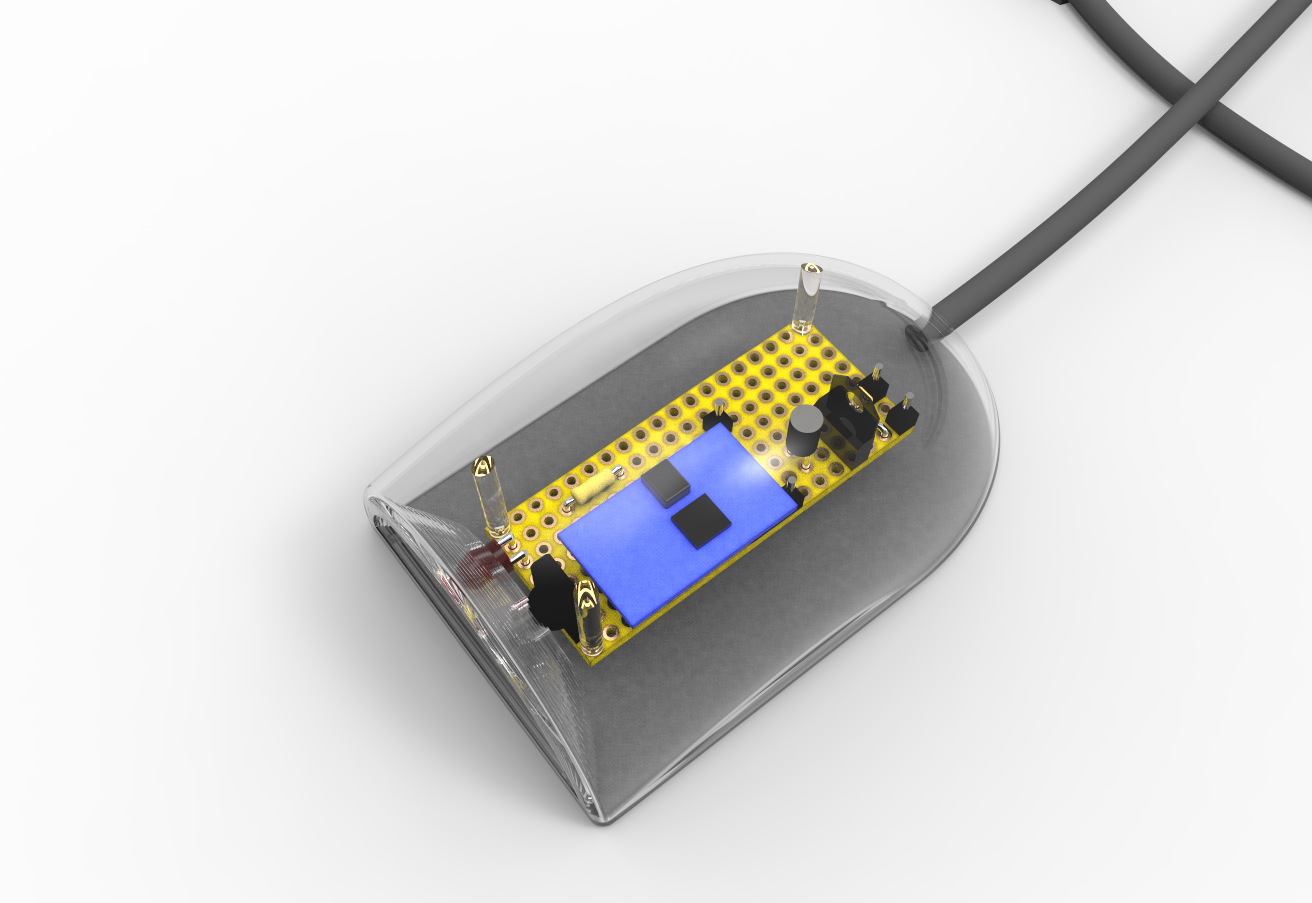
\includegraphics[width=13cm]{7_Live_Demo}
\end{minipage}
}

\end{document}


